\documentclass[11pt]{article}
\usepackage{amssymb,amsmath,amsthm}
\usepackage{amsmath,amssymb,enumerate}
\usepackage{xcolor}
\usepackage{tikz}
\usetikzlibrary{positioning,decorations.pathreplacing,quotes}
\usetikzlibrary{bayesnet}
\tikzset{tick/.style={draw, minimum width=0pt, minimum height=2pt, inner sep=0pt, label=below:$#1$},
    tick/.default={}}

\begin{document}

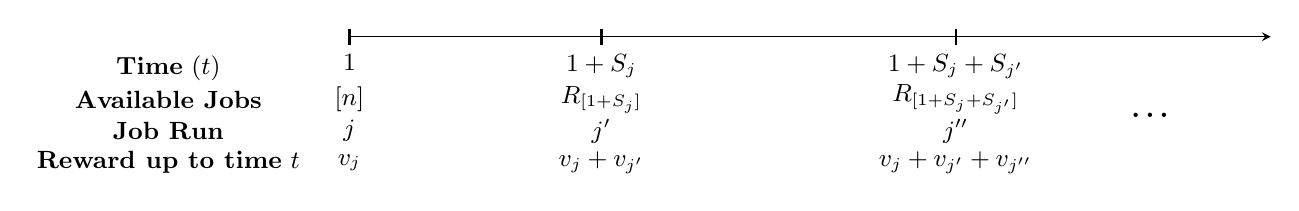
\begin{tikzpicture}
\draw [-stealth](2.3,0) -- (14,0);
\path (0, -0.4) node {\small \textbf{Time} $(t)$};
\path (0, -0.8) node {\small \textbf{Available Jobs}};
\path (0,-1.2) node {\small \textbf{Job Run}};
\path (0, -1.6) node {\small \textbf{Reward up to time} $t$};
\draw[thick] (2.3,0.1) -- ++ (0,-0.2) node[below] {\small $1$};
\path (2.3,-0.8) node {\small $[n]$};
\path (2.3,-1.2) node {\small $j$};
\path (2.3,-1.6) node {\small $v_j$};
\draw[thick] (5.5,0.1) -- ++ (0,-0.2) node[below] (U) {\small $1+S_j$};
\path (5.5,-0.8) node {\small $R_{[1+S_j]}$};
\path (5.5,-1.2) node {\small $j'$};
\path (5.5,-1.6) node {\small $v_{j}+v_{j'}$};
\draw[thick] (10,0.1) -- ++ (0,-0.2) node[below] (U) {\small $1+S_j+S_{j'}$};
\path (10,-0.8) node {\small $R_{[1+S_j+S_{j'}]}$};
\path (10,-1.2) node {\small $j''$};
\path (10,-1.6) node {\small $v_{j}+v_{j'}+v_{j''}$};
\path (12.5, -1) node{\textbf{\dots}};
%         (U.north -| END.north);
%         (U.south -| UU.south);
\end{tikzpicture}

\end{document}